\section{Numerical experiments}

To evaluate the simple model of \sref{model}, we conduct a battery of direct numerical simulations.
The novel components of the simple model, i.e. viscous drag and mixing, are most pronounced at late times.
We primarily direct our effort at simulating higher aspect ratio domains to allow the bubble to reach a dissipative regime.

The numerical experiments simulate the incompressible Navier-Stokes equations with the Boussinesq approximation:
\begin{align}
\frac{\partial u}{\partial t} + u \cdot \nabla u &= \nu \nabla^2 u - \nabla P + A g \phi \\
\frac{\partial \phi}{\partial t} + u \cdot \nabla \phi &= D \nabla^2 \phi 
\end{align}
where $u$ is the velocity,
$\nu$ is the kinematic viscosity,
$P$ is the pressure,
$\phi$ the non-dimensional density,
and $D$ is the diffusivity of $\phi$.

The initial conditions are quiescent with a horizontal interface perturbed by product of cosine functions and smeared by an error function:
\begin{equation}
\phi(x,y,z,t=0) = \text{erf}\left(\frac{z + a_0 \cos(2 \pi (x/\lambda)) \cos(2 \pi (y/\lambda))}{\delta})\right)
\end{equation}
where $a_0$ is the initial amplitude and $\delta$ is the initial interface thickness.
Both $a_0$ and $\delta$ are taken to be small enough to minimize their effects on the solution, $0.01$ and $1/???$, respectively.
The governing equations and initial condition have four dimensional parameters: $\nu$, $D$, $Ag$, $\lambda$.
These are combined into 2 non-dimensional numbers, the Grashof number and the Schmidt number:
\begin{equation}
\text{Gr} = \frac{A g \lambda^3}{\nu^2} \quad \text{Sc} = \frac{\nu}{D}
\end{equation}
The Grashof number serves the role of a Reynolds number for instability problems without a consistent characteristic velocity.
For this reason, the root of the Grashof number is sometimes called the \textit{perturbation Reynolds number}~\cite{Wei2011}:
\begin{equation}
\text{Re}_p = \sqrt{\frac{A g \lambda^3}{\nu^2}}
\end{equation}

The domain is $\left[0.5, 0.5, 64\right]$ and rotated 45 degrees to model $\lambda = \sqrt{2}$ with symmetric span-wise boundaries.
The length of the domain is $64/\sqrt{2} \approx 45.2$ wavelengths with no-slip walls at the top and bottom.
Based on a previous validation of the smRTI with no-slip boundaries, we expect the bubble to be unaffected by the top and bottom walls until it reaches 75\% of the height, or about $17\lambda$.
This provides significantly more data than the $h < 4 \lambda$ results of Ramaprabhu \etal~\cite{Ramaprabhu2012}.

The model introduced in \sref{model} assumes the bubbles and spikes are coherent structures, that is they travel at some velocity and have a well defined interface.
As the Grashof number increases and the bubbles and spikes break up, departing from the assumptions of the model.
On the other hand, at low Grashof number and finite diffusivity, diffusion moves the $\phi = 0$ interface, as opposed to simply transporting the scalar across it, which also departs from the model assumptions.
For these reasons, we restrict our study to an intermediate range of Grashof numbers: those which are large enough to sustain bubble dynamics while not being so large as to break the bubbles apart.
This range has been identified empirically to be approximately $??? \le \text{Gr} \le ???$ for Schmidt numbers greater than 1.

The number of spatial samples needed to resolve the advection-diffusion equation for the scalar goes with the Peclet number to the third power.
It is prohibitively expensive to perform calculations at high Schmidt numbers and high Grashof numbers.  
For this reason, we restrict the diffusivity to be no lower than ???, which provides $\text{Sc} = 4$ for the highest Grashof number in our range and higher for correspondingly lower Grashof numbers.

Simulations are performed with the NekBox version of the Nek5000 code, which has been previously validated against single-mode Rayleigh-Taylor experiments~\cite{Validation2016,Wilkinson2007}.
The spectral element method implemented by NekBox has purely dispersive errors and converges exponentially with the spectral order.
The the resolution parameters; the number of spectral elements, the order of the spectral elements, and the time step; were chosen to achieve an accuracy of $10^{-4}$ in the bubble aspect ratio~\cite{Convergence2016}.

\subsection{Observables}

\begin{figure}
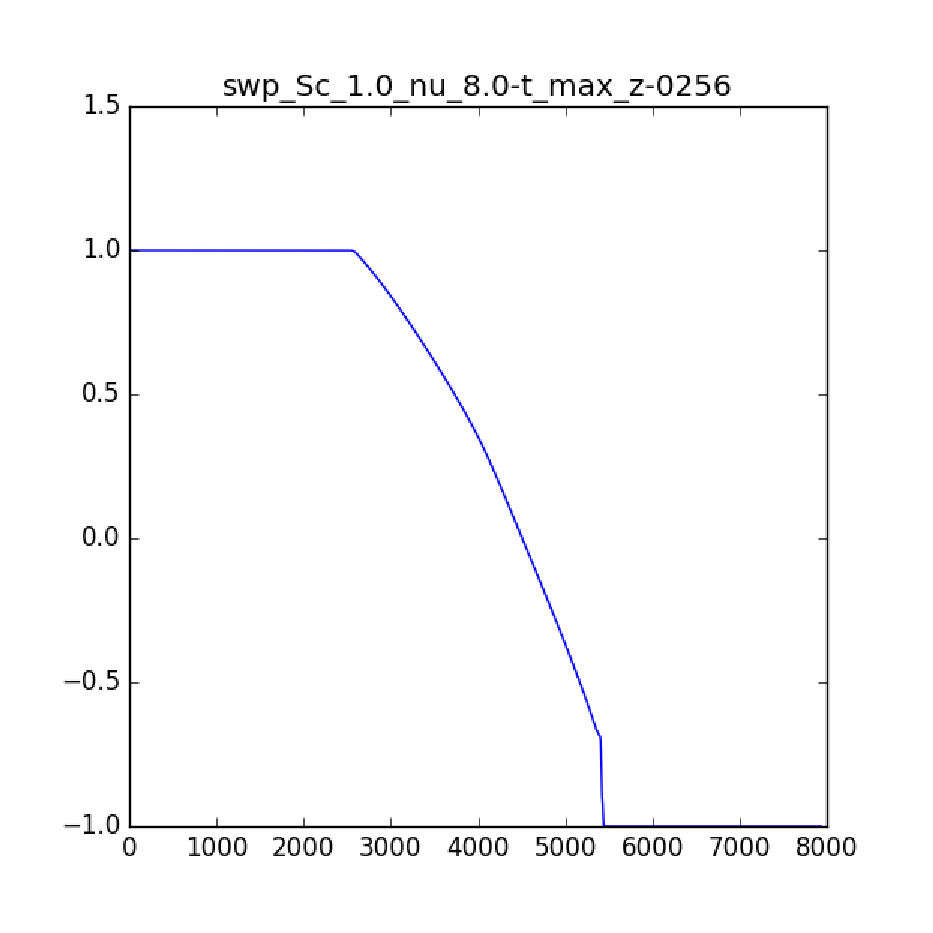
\includegraphics[width=\columnwidth]{figs/swp_Sc_1.0_nu_8.0-t_max_z-0256.eps}
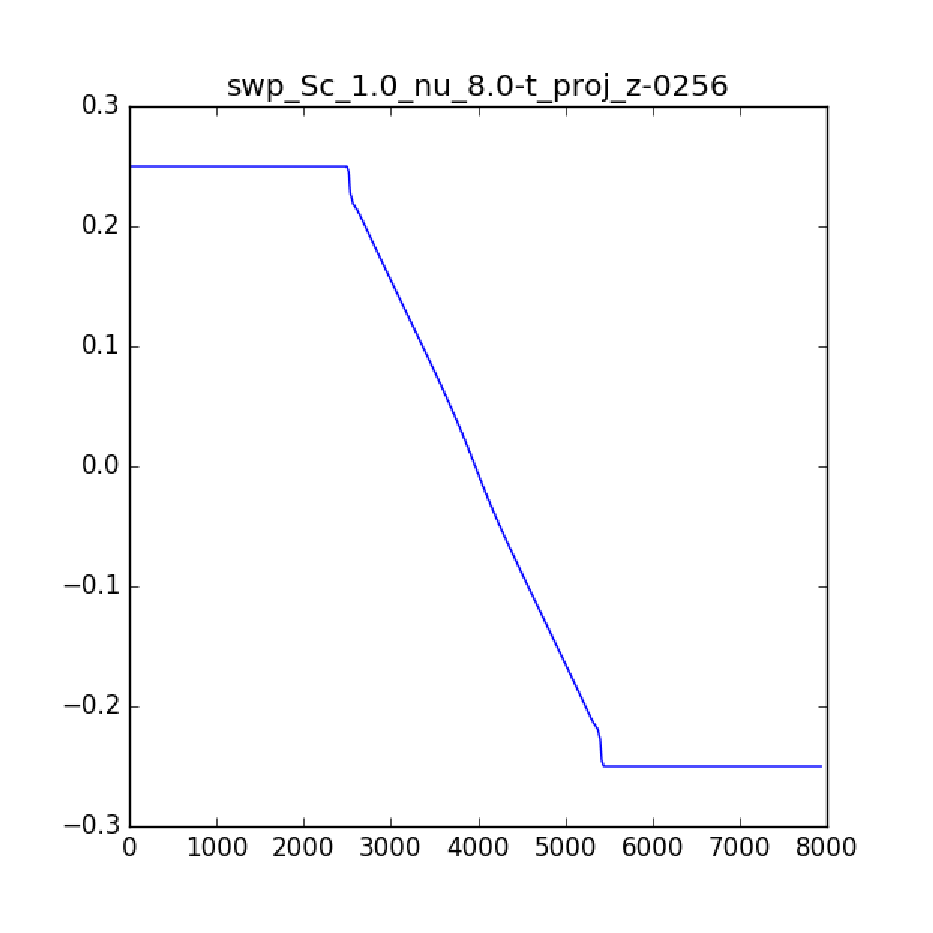
\includegraphics[width=\columnwidth]{figs/swp_Sc_1.0_nu_8.0-t_proj_z-0256.eps}
\caption{\flabel{profiles}
  Span-wise max and mean of scalar field.
}
\end{figure}

\begin{figure}
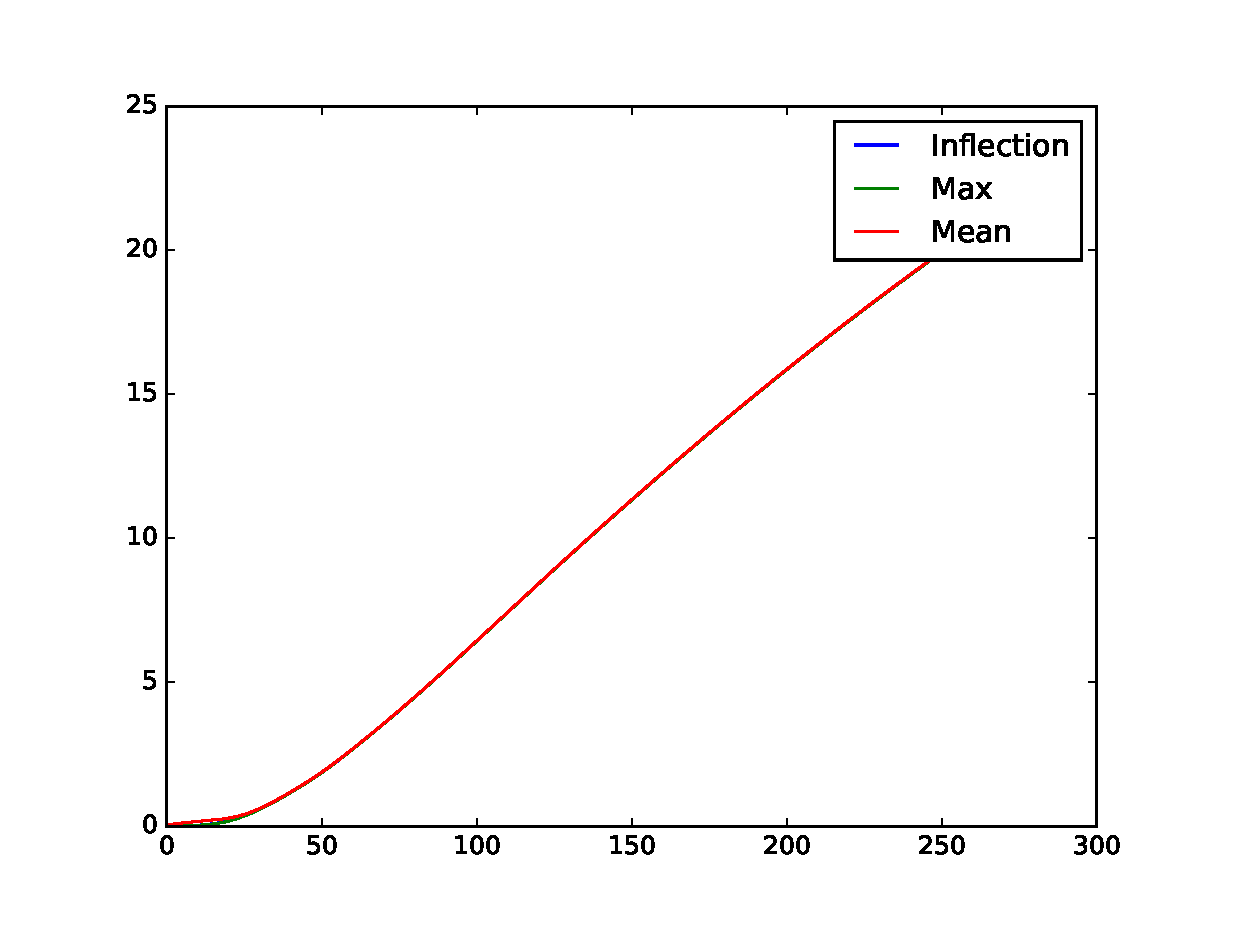
\includegraphics[width=\columnwidth]{figs/comp-height-0.0008-0.0002.eps}
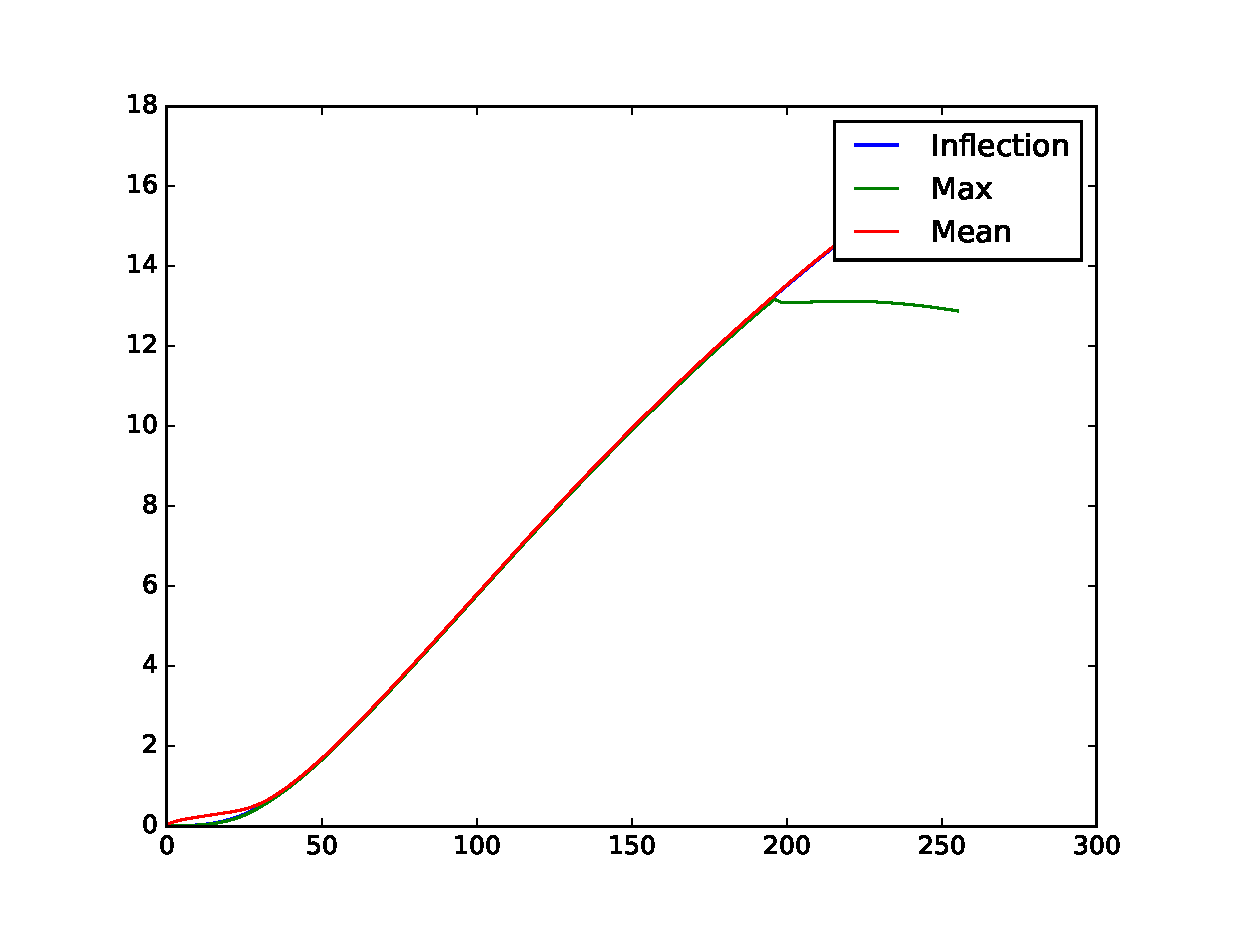
\includegraphics[width=\columnwidth]{figs/comp-height-0.0008-0.0004.eps}
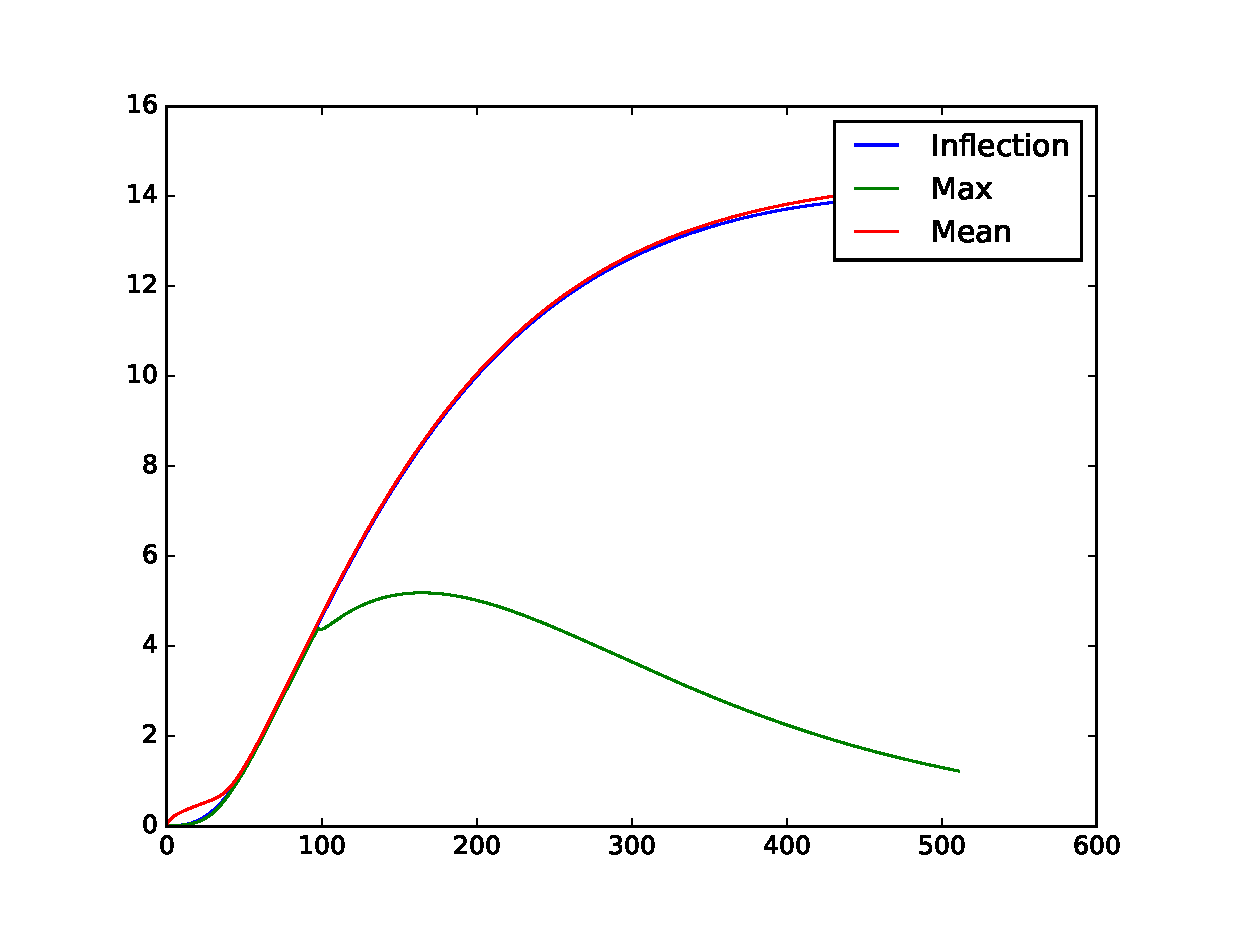
\includegraphics[width=\columnwidth]{figs/comp-height-0.0008-0.0008.eps}
\caption{ \flabel{heights}
  Comparison of height metrics at $\text{Gr} = ???$ and $\text{Sc} = \{2, 4, 8\}$.
}
\end{figure}

The output frames are post-processed, extracting 0, 1, and 2D projections of a variety of quantities along the axis, mid-plane, bubble cross section, etc.


\paragraph{Bubble height}
For miscible RTI, the shape of the profiles is due to a combination of advection in the bubble and diffusion across the interface.
We can assume an error function-like profile across the interface at the bubble tip, but diffusion across the bubble sidewalls results in a linear profile in both the span-wise mean and maximum.
To separate the definition of the bubble tip from the effect of decreasing effective Atwood number, we introduce a new definition: the bubble tip is defined as the inflection point in the span-wise maximum scalar profile.
For the symmetric case, this span-wise maximum of the scalar is equivalent to the value along the bubble axis.
At early times, the profile is an error function that broadens with diffusion and advects with the bubble velocity.
At late times, the $\phi > 0$ side of the error function decays into a nearly linear profile, as seen in \fref{profiles}.
However, the profile remains sharp near the bubble tip, decoupling the position of the inflection point from the sidewall mixing.

This definition of the bubble height is compared to two more traditional definitions, based on a cutoff in the mean or maximum profiles, in \fref{heights}.
At early times, the definition based on the mean profile grows diffusively.
At late times, the definition based on the max profile kinks as the linear part of the profile crosses zero and then stagnates.
The definition based on the inflection avoids both breakdowns while closely tracking each other definition in its valid range.

\paragraph{Mixed volume}

The scalar is normalized such that $\phi \in \left[-1, 1\right]$ and the average $\bar\phi = 0$.
The purity of the fluid is therefore $\left| \phi \right|$ and the volume of mixed fluid is given by a simple integral:
\begin{equation}
M(t) = \int \left( 1 - \left| \phi(x,y,z) \right|\right) dV
\end{equation}

